% --------------------------------------------------
% Literature Review
% --------------------------------------------------
% The literature review is an essential component of your project report. You should discuss the existing literature that is relevant to your project with full and proper referencing. You should aim to refer to a range of material including academic papers, text books, articles and existing product descriptions. It should be clear to the reader why the literature you identify is relevant and how you have incorporated the learnings from your review into your project. For example, you may have made a number of project 
% Page 4 of 5 decisions based on your review of the literature and these decisions should be described. The literature review should also lead to the creation of a number of possible solutions to your problem articulation and technical specification

\chapter{Literature Review} \label{lit}

This chapter examines various literature surrounding the project objectives stated in Section \ref{section:probart-techspec} with the purpose of gaining insight into the current state of the art and how other similar products function. It looks at the various methods of \textbf{Real-Time Communication} that exist in order to create an environment where feedback is fast and frequent \textit{(Section \ref{lit-rtc})}. It examines some \textbf{existing systems} that are providing some of the features listed and critically examines the positives and negatives of some of the technical choices that are apparent in these systems \textit{(Section \ref{lit-ode})}. It also analyses some of the modern advances in \textbf{Virtualisation} technology along with how the advent of \textbf{Containers} has changed the landscape of PaaS services and virtual environments in general \textit{(Section \ref{lit-containers})}. It concludes by looking at the state of the art in \textbf{front-end} \textit{(Section \ref{lit-front-end})} and \textbf{back-end} \textit{(Section \ref{lit-back-end})} technologies that can be used to create a modern web application. 

\section{Real-Time Communication} \label{lit-rtc}

Real-Time Communication (RTC) is an important research topic for this project in order to create an environment for users that feels as close to a local experience as possible. The requirement for fast feedback is essential.

An experiment carried out in 2012 discussing the performance of different RTC methods by Professors at the University of New Brunswick \cite{websocket}. This experiment compared the different standard HTTP methods of implementing Real-Time Communication against the new (at the time) technology of WebSockets which are designed to create a full duplex bidirectional data-flow.

\subsection{HTTP Polling}

\textbf{HTTP polling} is an attempt to solve the real-time issue by repeatedly making a request to a web server at a pre-determined time interval to check if there are messages waiting to be read. \textbf{HTTP long-polling} is another solution that uses the HTTP protocol but reduces the number of requests by having the server intelligently not respond to the request if there is no data available and hang until a timeout or information becomes available. Both of these solutions are inadequate for a responsive system because the HTTP protocol is still built on top of a system not designed for a real-time, full duplex communication channel. HTTP relies on a 'Request-Response' model which is only half duplex so polling was only a solution that worked for systems that were reliably sending data at a steady rate such as sensors that are being queried for an API.

\subsection{WebSockets}

A modern solution to the issues of HTTP polling is the \textbf{WebSocket} protocol proposed in RFC 6455 \cite{wsrfc} which aimed to reduce latency by a factor of three compared to HTTP in the real-time communication aspect. It is a full duplex, bidirectional communication channel that provides an efficient method of communicating between several different clients using a persistent connection between the client and the server. A client may connect to a websocket endpoint on the server, send messages to it, and the server may broadcast messages back to just that client or to every client connected. Due to this behaviour it is very popular for creating text based chat communication systems.

WebSockets work by utilising a persistent TCP connection where messages can be sent back and forth without requiring a new connection be made every time \cite{wsrfc}. This behaviour is possible in HTTP since HTTP 1.1 however, WebSockets do not adhere to the 'Request-Response' format that a HTTP request utilises. Any client connected to the socket is capable of broadcasting a message at any time. HTTP persistent connections also still suffer from latency due to the effort the protocol makes to control congestion \cite{httpvsws}. WebSockets take the concept further by making it simple to embed data with each request in the form of a JSON schema based string. This makes it ideal for the transfer of small chunks of text where the only data is the required form of the response. WebSockets are not appropriate for downloading resources or assets such as images.

\begin{figure}[h!]
    \centering
    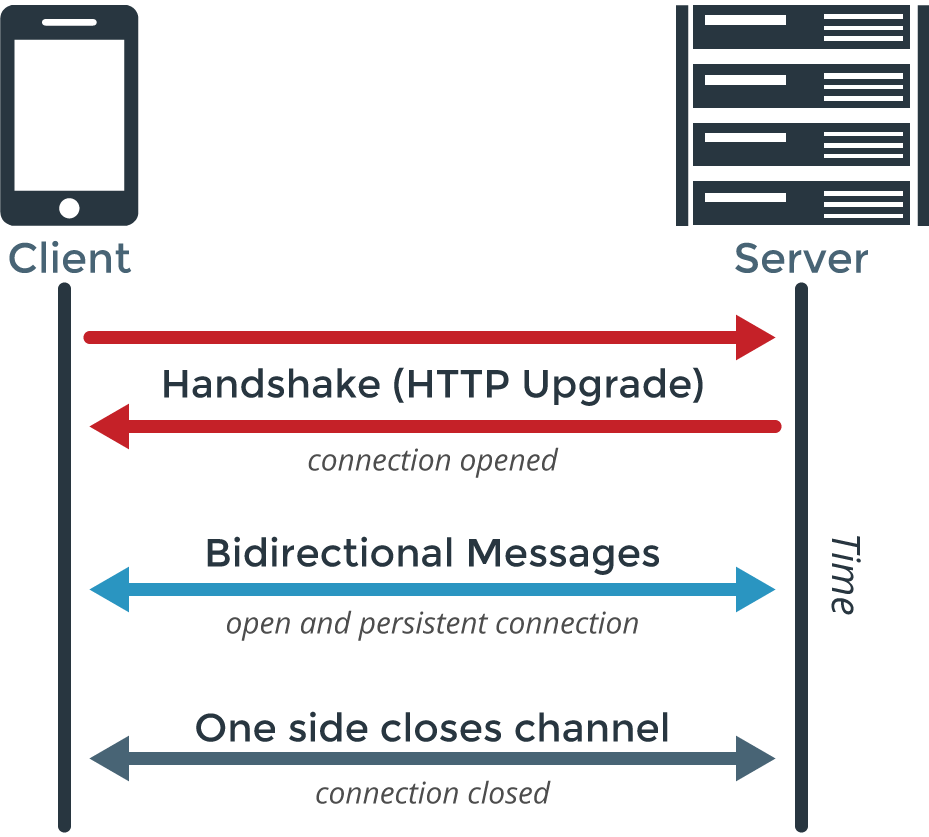
\includegraphics[scale=0.3]{res/WebSockets-Diagram.png}
    \caption{Illustration of WebSocket connection \cite{websocket-img}}
    \label{}
\end{figure}

\subsection{Web RTC}

Another new approach of RTC on the web has been developed by Google in collaboration with other browser vendors called \textbf{WebRTC} \cite{webrtc}. This technology is focused on streaming audio and video between different clients on the web. This new technology is aiming to be the replacement for the browser plugins that have been necessary in order to use P2P video/voice chat software such as \textit{Skype, Facebook Messenger, Google Hangouts, etcetera} \cite{webrtc}. WebRTC is more appropriate for applications that need a streaming based connection as it's latency is even lower than WebSockets due to it utilising the UDP protocol which has much less overhead compared to the TCP based connection of WebSockets \cite{udpvstcp}. WebRTC would not be appropriate for the use case of WebSockets when transferring informational data between clients, such as a chat application. It is important to make sure that the data is being received in the correct order whereas UDP is less concerned as long as enough packets get transferred to create a stable audio/video connection.

\section{Virtual Machines and Containers} \label{lit-containers}

To meet the objective of providing as close to local an experience as possible to the users of the system, a virtual environment for executing code and saving files is vital. Virtualisation technology is changing significantly due to the different container based-solutions which attempt to promote a more disposable and lightweight type of virtual environment compared to  hypervisor powered alternatives.

\subsection{Virtual Machines}

Virtualisation is a technique in computing that most commonly is seen by users via the use of desktop \textbf{Virtual Machine} (VM) software. Virtual Machines are heavily utilised to provide virtual desktop environments on top of a users host operating system. The advantages of Virtual Machines are a sandbox environment for potentially harmful operations, such as when penetration testers are trying to fingerprint a virus. The option of trying different operating systems without needing to dedicate a partition of disk space or deal with a dual booting set up is another user facing benefit of virtual machines.

In the enterprise world, Virtual Machines are being used to host customers applications in a full Platform-as-a-Service (PaaS) solution so customers no longer have to worry about hosting their own web servers or other online services. %TODO: reference

The general way of interacting with fully virtualised environments is through a hypervisor which is a process that is responsible for provisioning and monitoring Virtual Machines \cite{hypervisor}. The hypervisor allocates resources such as memory and CPU cores from the host machine that the VM is allowed to consume. When the VM is shut down these resources are freed and can be used by the host system once again. The hypervisor also allows the VM to use a different base operating system than the one that is on the host machine as it provides a complete comulation of a computer system

\subsection{Containers}

Containers are a much lighter virtualisation technology than  Virtual Machines despite the functionality being similar. They achieve this as they are much closer to the systems 'bare metal' as any commands that are executed through a container are running on the host's hardware and kernel. This means that there is no need for a hypervisor as containers have direct access to the system resources. Usage limits can be applied to container based process.

As containers traditionally don't utilise a hypervisor the biggest difference between them is that the engine that powers the container provisioning software such as the \textit{Docker Engine} isn't able to virtualise an environment based on a different OS. This is more by design however as it is what gives containers their 'lightweight' quality as they aren't having to simulate the kernel. Not having a full emulated computer system and kernel to boot means that containers can start up significantly faster than a VM.

\begin{figure}[h!]
    \centering
    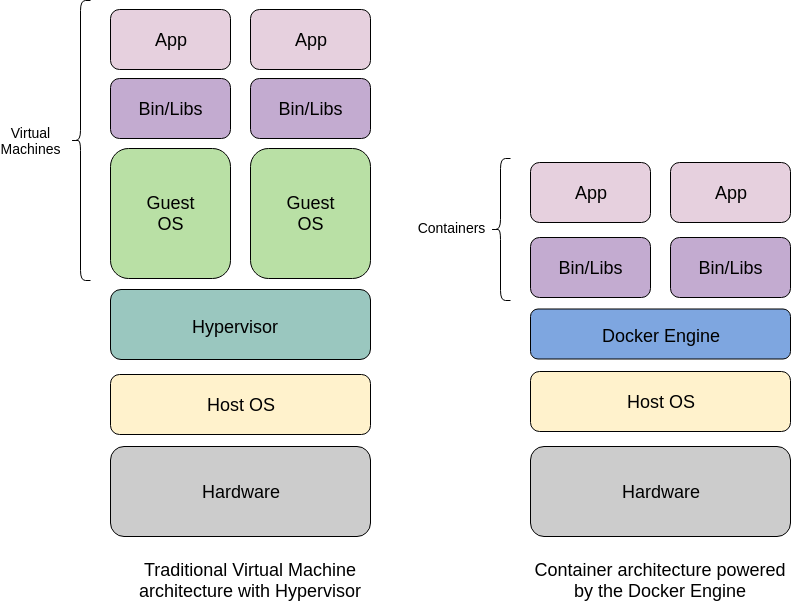
\includegraphics[scale=0.4]{res/Virtualisation.png}
    \caption{Architecture of Virtual Machines vs. Containers}
    \label{fig:architecture}
\end{figure}

Due to their performance benefits containers have become popular options for PaaS software. A paper was written comparing the benefits of a fully virtualised environment against a container based solution \cite{contsvsvirt}. It concluded that containers have an inherent advantage over VMs due to the performance benefits and the quick start up time of them. It also mentions that few PaaS vendors are using containers for their systems so far as they are too new of a technology. It is worth nothing that the report was published in 2014 however and since container technology usage has increased dramatically \cite{container-report}.

\section{Container Providers}

As containers are a more modern innovation than hypervisors, there has been a recent wave of different technologies that attempt to make simple containers in varying ways.

\subsection{Linux Containers}

As mentioned above, \textbf{Linux Containers} or \textbf{LXC} are the foundation of many container solutions. This is due to the fact that they offer a lightweight kernel implementation which provides every container with some key features.

\begin{itemize}
    \item A unique Process ID per container
    \item Isolates all resources for the container by using cgroups and namespaces
    \item Provides each container with it's own private IP address
    \item Isolates all files on the container from the Host by using chroot
\end{itemize}

The features listed above are all features standard in the Linux kernel. \texttt{cgroups} \cite{cgroups-man} or control groups are a feature that is able to isolate and allocate resources from the machine to each individual process. 

\texttt{namespaces} \cite{namespaces-man} is another key feature of the kernel which LXC relies on in order to provide isolation to each container. The purpose of namespaces is to wrap a process or a group of processes in an isolated instance of the global resource. Changes of global resource to other processes aren't visible to other namespaces.

In terms of downsides the LXC implementation is heavily tied to the Linux OS which means that it is not possible to run it on a different OS such as Windows. There are also some security concerns for LXC as all containers share the one host kernel.

\subsection{OpenVZ Containers}

OpenVZ makes use of a modified Linux kernel with it's own set of extensions. OpenVZ is able to manage physical and virtual servers with \textit{dynamic real-time partitioning}. It similarly offers better performance than a traditional hypervisor based system and utilises the cgroups and namespaces features of Linux to provide it's virtual environments.

On top of the advantages of LXC it also provides the following benefits.

\begin{itemize}
    \item \textbf{Container Lifecycle} remote management can be done of containers using an API to modify the status of a container in real-time. 
    \item \textbf{Container State} is able to create checkpoints during the container's lifecycle so that it may be recovered from that point should anything go wrong.
\end{itemize}

These mean that there is greater user access over the state of containers and that restoration points can be created to store users progress with a container.

\subsection{Docker}

The Docker process is a daemon which can provide and manage Linux Containers as \textit{images}. It uses LXC for the container implementation and then adds on top an image management system which makes use of a \textit{Union File System} \cite{contsvsvirt}.

Using the daemon, Docker manages to provide similar functionality as the OpenVZ containers in relation to lifecycle and state. The state of a container at any time can be saved to a new image which can then be reloaded by the daemon to the same point

Unlike OpenVZ, Docker can be run with the standard Linux kernel and therefore is more suited for PaaS software. It also has a thriving ecosystem of pre-made images which offer a huge array of different starting points and tools \cite{dockerhub}.

\section{Online Developer Environments} \label{lit-ode}

A number of existing solutions providing online development environments exist and have been analysed for the purpose of this review.

\subsection{Repl.it}

Repl.it is very similar to the idea proposed in the Problem Statement (Section \ref{section:probart-probstate}) and a lot of the requirements lined out in Section \ref{section:probart-techspec}. It offers a large array of Repl templates available for users to get started with many languages/frameworks very quickly. It also uses the Monaco Editor provided by Microsoft in order to provide a first class text editor experience.

Repl.it takes advantage of containers in order to gives users a full developer experience when using the system \cite{replit-containers}. The system also uses its own container orchestration software in order to scale the instances available to users up and down based on current and predicted demand.

Every code result is available to be viewed/run through a special \texttt{.repl.run} subdomain. This includes long running processes like web servers which are able to be hosted from these subdomains and be always accessible. This means you could create several REPLs which can all inter-connect to each other like a full system.

Technically the system is impressive. Something that the system doesn't recreate quite as smoothly as a local environment is a small amount of latency between keys being pressed and the corresponding value appearing in the REPL itself.

The system also seems to remove all previously typed entries of the REPL on every press of the \textit{Run} button. This suggests that it is giving you a new REPL instance on every execution which isn't how a local environment works.

From a HCI point of view the website feels very smooth to use and is not frustrating other than the latency noted when typing directly into the running container via the REPL.

Repl.it is clearly very focused on the objective of replacing local development environments and does a good job of fulfilling that need.

\subsection{Codecademy}
Codecademy is a education focused online environment designed to teach users how to code. Ranging in topics from beginning web development to a course on the IBM Watson API. It is a more directed experience than Repl.it as users are performing tasks for exercises but they are typing code into a similar environment, the code is executed and the result is displayed to the user.

Codecademy does not allow access directly to the REPL but if code is entered into the editor which allows for user input such as the \texttt{input()} function in Python, then it interprets the input correctly.

The Codecademy web application is clearly a complicated system and it shows by how unresponsive it feels when navigating from page to page. The page does a full reload even though there are elements which do not change on the screen. This leads to a frustrating pause and blank screens between page loads.

It is clear that Codecademy is a focused environment to encourage new developers to get into development by offering an easy to start environment and heavily directed experience. It is not concerned with the idea of replacing local development environments so much as making sure that it's not something beginners should need to think of when wanting to learn a new tool.

\subsection{Glitch}
Glitch is a web application that is focused on trying to cultivate a social coding community that encourages developers to help each other out and build mini applications with JavaScript and Node.js. It provides an online coding environment that uses containers to isolate the users runtime.

Glitch is focused heavily on the social aspect. On the homepage they have a section dedicated to users asking for help so more experienced developers can help them achieve their goals with the applications they want to build. It also showcases user made projects on the homepage which can be \textit{Remixed} which is similar to forking a repository on GitHub for other users to modify.

In terms of design, the website has a very colourful friendly interface. A feature which is particularly notable is in each project editor there is an option to view \textit{Container Stats} where the CPU usage is shown as a percentage, Memory usage in bytes and additional relevant information can be found. There are also guidelines on the technical restrictions for projects that are run in Glitch. 

\section{Front-end Web Technologies} \label{lit-front-end}

The client side of web applications is based on three fundamental technologies, \texttt{HTML}, \texttt{CSS} and \texttt{JavaScript} which declare both the layout of the application and the functionality.

Web development has changed greatly since its inception and new technology has been released that gives developers greater flexibility in how they build their modern web apps. Since the creation of jQuery \cite{jquery} a number of JavaScript based frameworks/libraries have been released that try to solve some of the problems that are inherent to the web platform.

\subsection{React}

React was developed by Facebook and attempts to simplify the process of creating interactive UIs by providing a declarative way of writing user interfaces and encouraging the reuse of \textit{components} which are composed HTML elements with the ability to provide interaction through JavaScript.

The need for a library such as React comes from the difficulty involved with maintaining state between what is displayed on the screen and variables that exist in the JavaScript code-base. React also offers a high amount of code reuse with its component architecture. 

React is able to use JavaScript functionality inline with HTML style layout syntax via use of JSX (a syntax extension to JavaScript) and a transpiler which converts JSX into React api function calls at build time.

React has a very strong community with over 80,000 packages listed on the npm package registry \cite{npm-search-react}.

\subsection{Vue.js}

Vue.js is a JavaScript Framework that offers a lot of the same functionality as React but offers it in a way that is more akin to the traditional way that web development is done. Where React blends the 3 key technologies of the web into a JavaScript focus. Vue.js maintains a separation of these concepts.

Vue.js offers more than React out of the box such as an official routing solution for single page applications, global state management and server side rendering.

Vue uses ordinary HTML as it's view templating however it is able to inject it's own directives and JavaScript functionality by making use of the popular handlebars syntax.

It has grown very quickly since it came out in 2014 and has just over 25,000 packages published on npm \cite{npm-search-vue}.

\section{Back-end Technologies} \label{lit-back-end}

There are numerous tools in use both professionally and recreationally to create web servers, databases, and other tools that a system might need to utilise. 

Traditionally, the back-end of an application was written in a language such as \texttt{PHP} or \texttt{C\#}. In more recent times however, there has been a rise of more developer friendly scripting languages such as \texttt{Python} or \texttt{JavaScript} which are powering infrastructure for some of the biggest technology companies in the world.

\subsection{Node.js}
Node.js \cite{nodejs} is a JavaScript runtime built on top of Google's Chrome V8 engine. As JavaScript is a single threaded language many thought it was unsuited to hosting back-end applications due to the lack of concurrency features. Node.js uses the \texttt{libuv} C library \cite{libuv} in order to create an event loop which has the task of offloading external functions such as network I/O. When a response is received the event loop can pass the result back to the JavaScript environment. This is how Node.js is made to be a scalable and viable option for hosting servers and running in a browser-less environment.

Node.js is in wide use in the industry with companies such as Netflix \cite{netflix-nodejs} making widespread use of the platform which is testament to how powerful it can be even at huge scale. Node.js is also appropriate for use where the application is smaller in scale and perhaps only needs to interact with external processes and host a small number of endpoints.

\subsection{.NET Core}

.NET Core \cite{.netcore} is a cross platform framework developed by Microsoft which can be used to develop large scale web applications. 

.NET Core is able to provide a full stack set of features relying on Model-View-Controller architecture where the Models and Controllers are written in any Common Intermediate Language (CIL) based langauge and the views are written in Microsoft's Razor syntax which is similar in idea to React or Vue's templating/JSX but uses C\#.

Being supported and created by Microsoft means that it's extremely useful for the type of applications that large enterprises regularly develop.

\pagebreak
